\documentclass[aspectratio=169]{beamer}
\usetheme{Madrid}
\usecolortheme{default}

\usepackage{amsmath}
\usepackage{amssymb}
\usepackage{graphicx}
\usepackage{physics}
\usepackage{booktabs}
\usepackage{bm}
\usepackage{multicol}
\usepackage{tikz}
\usepackage{circuitikz}
\usetikzlibrary{positioning}
\usepackage[backend=biber,style=numeric]{biblatex}

\usepackage{tikz}
\usepackage{circuitikz}

% \title[DeepMD–HALMD Integration]{Integration of Deep Potential Molecular Dynamics (DeepMD v2) into HALMD for Multi-Species Alloy Systems}
\title[DeepMD–HALMD Integration]{Accurate implementation of DeepMD-v2 potential calculation in HALMD for single species, extension to multi-species and Automatic-Differentiation-Based Force Computation}

\author{Sandip Kumar Sah}
\institute{M.Sc. Computational Science, Freie Universität Berlin }
\date{\today}

\addbibresource{ppt_ref.bib}


\begin{document}

%=====================================================
% \begin{frame}
% \titlepage
% \end{frame}
\begin{frame}
  \titlepage
  \vspace{1cm}
  \begin{center}
    \large \textbf{Supervisor:} Prof. Dr. Felix Höfling
  \end{center}
\end{frame}

%=====================================================
\begin{frame}[allowframebreaks]{Content}
\setcounter{tocdepth}{2}
\begin{multicols}{2}
\tableofcontents
\end{multicols}
\end{frame}

\section{Introduction}
%=====================================================
\subsection{Motivation}

\begin{frame}[allowframebreaks]{Motivation}
\begin{itemize}
    % \item MD relies on interatomic potentials to approximate quantum-mechanical interactions \cite{frenkel2023understanding}.
    
    \item Classical potentials are efficient but inaccurate for complex chemistry, while \textit{ab initio} methods are accurate but computationally expensive \cite{daw1984eam,marx2009ab}.
    
    \item Machine-learned potentials (e.g., DeepMD) achieve near--DFT accuracy at classical MD cost \cite{behler2007generalized,wang2018deepmd}.
    
    \item Current DeepMD--HALMD integration is limited to single-species systems \cite{cruz2025deepmd}.
    
    \item This thesis enables scalable, accurate multi-species DeepMD simulations in HALMD.
\end{itemize}
\end{frame}



%=====================================================
\subsection{Objectives and Scope}

\begin{frame}{Objectives and Scope}
\begin{itemize}
    \item Extend the DeepMD integration in HALMD beyond the single-species implementation of Cruz to full \textbf{multi-species DeepMD-v2} inference \cite{cruz2025deepmd}.
    
    \item Implement the missing core components of the DeepMD-v2 pipeline:
    \begin{itemize}
        \item periodic coordinate handling, ghost atoms, and multi-type neighbor lists,
        \item species-dependent filter and descriptor networks,
        \item normalization, scaling, smooth cutoffs, and accurate force backpropagation
    \end{itemize}
    \cite{wang2018deepmd,zeng2023deepmdv2}.
    
    \item Focus on the \textbf{inference stage} (energy and force evaluation) for multi-component materials using the DeepPot-SE descriptor; model training and alternative descriptors are outside the scope.
\end{itemize}
\end{frame}


%=====================================================
\section{Background}
\subsection{HALMD}
\begin{frame}{HALMD: High-Accuracy Large-Scale MD Engine}
\begin{itemize}
    \item HALMD is a high-performance, open-source MD framework for large-scale simulations, optimized for numerical accuracy and GPU acceleration \cite{colberg2011highly}.
    
    \item Atomic motion follows Newton’s equations of motion:
    \[
        m_i \frac{d^2 \mathbf r_i}{dt^2} = - \nabla_i U(\mathbf r_1, \mathbf r_2, \ldots, \mathbf r_N),
    \]
    
    \item Traditionally uses efficient empirical interatomic potentials, which are limited for complex chemistry \cite{daw1984eam,brenner2002reactive}.
    
    \item This thesis extends HALMD with multi-species DeepMD-v2 force fields, enabling near \textit{ab initio} accuracy at classical MD cost \cite{wang2018deepmd,zeng2023deepmdv2}.
\end{itemize}
\end{frame}



\subsection{DeepMD v2}



\begin{frame}{Neural Network Potentials and Deep Potential MD(DeepMD)-v2}
% \begin{frame}[allowframebreaks]{Neural Network Potentials \& DeepMD-v2}
\begin{itemize}
    \item \textbf{Neural Network Potentials} learn interatomic interactions from \textit{ab initio} data, achieving near--DFT accuracy at classical MD cost \cite{behler2007generalized,noe2020mlreview}.
    
    \item Energy is written as a sum of atomic contributions:
    \[
        E = \sum_i E_i(\mathcal{R}_i),
    \]
    ensuring locality and linear scaling \cite{behler2007generalized}.
    
    \item \textbf{DeepMD-v2}: modern NNP with smooth, symmetry-preserving descriptors, explicit multi-species support, and efficient GPU execution \cite{wang2018deepmd,zeng2023deepmdv2}.
    
    \item Species-specific embedding and fitting networks predict energies; forces follow from
    \[
        \mathbf F_i = -\frac{\partial E}{\partial \mathbf r_i}.
    \]
\end{itemize}
\end{frame}



%=====================================================

\section{Methodology}
\subsection{Overview of Implementation}
\begin{frame}{Overview of Implementation}
\begin{itemize}
    \item DeepMD-v2 is integrated into HALMD through a modular, end-to-end inference pipeline.

    \item Model parameters are extracted from \texttt{frozen\_model.pb} and \texttt{input.json} and converted into a compact HDF5 format for efficient loading.

    \item HALMD reconstructs local atomic environments using the exact DeepMD-v2 convention:
    \begin{itemize}
        \item periodic coordinate wrapping,
        \item ghost-cell extension,
        \item species-ordered neighbor selection.
    \end{itemize}

    \item From the reconstructed environment, HALMD computes descriptors and evaluates species-specific neural networks to obtain atomic energies and forces.
\end{itemize}
\end{frame}

\begin{frame}{DeepMD--HALMD Energy Evaluation Pipeline}
    \begin{figure}[H]
    \centering
    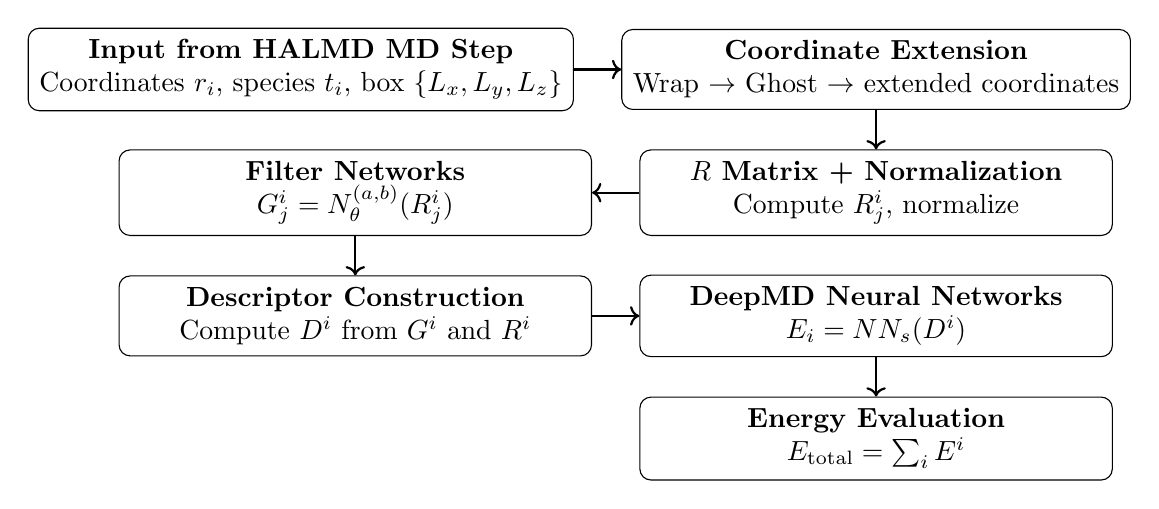
\begin{tikzpicture}[
        node distance=0.5cm and 0.6cm,
        box/.style={
            draw,
            rectangle,
            rounded corners,
            align=center,
            minimum width=6cm,
            minimum height=1.0cm,
            inner sep=4pt
        },
        arrow/.style={->, thick}
    ]

    % Row 1
    \node[box] (input) {%
    \textbf{Input from HALMD MD Step}\\
    Coordinates $r_i$, species $t_i$, box $\{L_x,L_y,L_z\}$
    };

    \node[box] (env) [right=of input] {%
    \textbf{Coordinate Extension}\\
    Wrap $\rightarrow$ Ghost $\rightarrow$ extended coordinates 
    };

    % Row 2
    \node[box] (R) [below=of env] {%
    \textbf{$R$ Matrix + Normalization}\\
    Compute $R^i_{j}$, normalize
    };

    \node[box] (filter) [left=of R] {%
    \textbf{Filter Networks}\\
    $G^i_{j} =N_{\theta}^{(a,b)}(R^i_{j})$
    };

    % % Row 3
    % \node[box] (G) [below=of filter] {%
    % \textbf{$G$ Matrix Construction}\\
    % Assemble $G_{ij}$
    % };

    \node[box] (D) [below=of filter] {%
    \textbf{Descriptor Construction}\\
    Compute $D^i$ from $G^i$ and $R^i$
    };

    % Row 4
    \node[box] (nn) [right=of D] {%
    \textbf{DeepMD Neural Networks}\\
    $E_i = NN_s(D^i)$
    };

    \node[box] (energy) [below=of nn] {%
    \textbf{Energy Evaluation}\\
    $E_{\text{total}} = \sum_i E^i$
    };



    % Arrows
    \draw[arrow] (input) -- (env);
    \draw[arrow] (env) -- (R);
    \draw[arrow] (R) -- (filter);
    % \draw[arrow] (filter) -- (G);
    \draw[arrow] (filter) -- (D);
    \draw[arrow] (D) -- (nn);
    \draw[arrow] (nn) -- (energy);


    \end{tikzpicture}
    \caption{DeepMD--HALMD energy evaluation pipeline implemented in this thesis.}
    \end{figure}


\end{frame}


\subsection{Model Parameter Extraction}
\begin{frame}{Model Parameter Extraction}
\begin{itemize}
    \item DeepMD-v2 models are stored as \texttt{frozen\_model.pb} with hyperparameters in \texttt{input.json} \cite{wang2018deepmd,zeng2023deepmdv2}.

    \item All parameters are extracted from the TensorFlow graph and converted into a compact HDF5 format for efficient inference in HALMD.

    \item The extracted model contains:
    \begin{itemize}
        \item descriptor attributes (cutoffs, normalization, species mapping),
        \item species-dependent embedding (filter) networks,
        \item species-dependent fitting networks,
        \item final outputs: energies, forces, and virials.
    \end{itemize}

    \item The hierarchical HDF5 model enables full multi-species DeepMD-v2 inference in HALMD, without TensorFlow, extending earlier single-species implementations \cite{cruz2025deepmd}.
\end{itemize}
\end{frame}


\subsection{Coordinate System Extension}

\begin{frame}{Coordinate System Extension}
\begin{itemize}
    \item \textbf{Problem:}  
    HALMD’s native neighbor handling uses the \textit{minimum-image convention}, sufficient for classical MD, but incompatible with DeepMD’s descriptor construction \cite{colberg2011highly,wang2018deepmd,zeng2023deepmdv2}.

    \item \textbf{DeepMD Requirement:}  
    Descriptors are computed from \emph{absolute atomic coordinates} inside the primary cell, requiring explicit:
    \begin{itemize}
        \item coordinate wrapping,
        \item ghost-cell periodic expansion,
        \item species-aware neighbor organization,
        \item descriptor normalization.
    \end{itemize}

    \item \textbf{Implemented Solution:}  
    A new DeePMD-style environment constructor that exactly reproduces the DeepMD-v2 preprocessing pipeline, replacing HALMD’s original environment construction \cite{cruz2025deepmd}.

    \item \textbf{Impact:}  
    Enables correct descriptor evaluation and full compatibility with multi-species DeepMD-v2 models.
\end{itemize}
\end{frame}


\begin{frame}{Explicit Coordinate Wrapping}
\begin{itemize}
    \item DeepMD requires all atoms to be mapped into the primary cell using fractional coordinates:
    \[
        \mathbf{s}_i = \mathbf{r}_i \mathbf{H}^{-1}, \qquad
        \tilde{\mathbf{s}}_i = \mathbf{s}_i - \lfloor \mathbf{s}_i \rfloor, \qquad
        \tilde{\mathbf{r}}_i = \tilde{\mathbf{s}}_i \mathbf{H}.
    \]

    \item This procedure is mandatory for general (non-orthorhombic) simulation cells and matches DeepMD’s internal pipeline \cite{wang2018deepmd}.
\end{itemize}

\vspace{0.3cm}
% \begin{center}
%     \begin{figure}[H]
%     \centering
%     \resizebox{1\textwidth}{!}{%
%     \begin{circuitikz}[transform shape]
%     \tikzstyle{every node}=[font=\tiny]

%     % Outer reference region
%     \draw [dashed] (-2,2) rectangle (2,-2);

%     % Primary simulation cell
%     \draw (-1,1) rectangle (1,-1);

%     % --- Real atoms r_i ---
%     \draw  (-1.5,1.5) circle (0.08cm) node[left] {$r_0$, $\tilde r_0$};
%     \draw  (1.5,1.5) circle (0.08cm) node[right] {$r_3$, $\tilde r_3$};
%     \draw  (-1.5,-1.5)  circle (0.08cm) node[left] {$r_1$, $\tilde r_1$};
%     \draw [dashed] (3.2,-0.5) circle (0.08cm) node[right] {$r_2$};

%     % --- Fractional coordinates s_i ---
%     \draw [dashed] (-0.75,0.75) circle (0.08cm) node[left] {$s_0$, $\tilde s_0$};
%     \draw [dashed] (0.75,0.75)  circle (0.08cm) node[below] {$s_3$, $\tilde s_3$};
%     \draw [dashed] (-0.75,-0.75)  circle (0.08cm) node[left] {$s_1$,$\tilde s_1$};
%     \draw [dashed] (1.6,-0.25) circle (0.08cm) node[right] {$s_2$};

%     % --- Wrapped fractional coordinates
%     \draw (0.6,-0.25) circle (0.08cm) node[above] {$\tilde s_2$};

%     \draw (1.2,-0.5) circle (0.08cm) node[above] {$\tilde r_2$};

%     % --- Mapping arrows ---
%     \draw[->, thin, gray] (-1.5,1.5) -- (-0.75,0.75);
%     \draw[->, thin, gray] (1.5,1.5) -- (0.75,0.75);
%     \draw[->, thin, gray] (-1.5,-1.5) -- (-0.75,-0.75);
%     \draw[->, thin, gray] (3.2,-0.5) -- (1.6,-0.25);

%     \draw[->, thin, blue] (1.6,-0.25) -- (0.6,-0.25);

%     \draw[->, thin, red] (0.6,-0.25) -- (1.2,-0.5);
%     \draw[->, thin, red] (-0.75,0.75) -- (-1.5,1.5);
%     \draw[->, thin, red] (0.75,0.75) -- (1.5,1.5);
%     \draw[->, thin, red] (-0.75,-0.75) -- (-1.5,-1.5);

%     % --- Axis guides ---
%     \draw [dashed] (-2,0) -- (2,0);
%     \draw [dashed] (0,-2) -- (0,2);

%     % --- Dimensions ---
%     \draw [<->, >=Stealth] (-2,2) -- (-2,-2) node[pos=0.5, fill=white] {$L_y=4$};
%     \draw [<->, >=Stealth] (-2,2) -- (2,2) node[pos=0.5, fill=white] {$L_x=4$};

%     \draw [<->, >=Stealth] (-1,1) -- (-1,-1) node[pos=0.5, fill=white] {2};
%     \draw [<->, >=Stealth] (-1,1) -- (1,1) node[pos=0.5, fill=white] {2};

%     \end{circuitikz}
%     }%
%     \caption{Explicit coordinate wrapping illustrated in stages: real coordinates $r_i$, fractional coordinates $s_i=\mathbf r_i \mathbf H^{-1}$, and wrapped fractional coordinates $\tilde s_i$.}
%     \label{fig:coordinate_wrapping}
%     \end{figure}
% \end{center}
\end{frame}


\begin{frame}{Explicit Coordinate Wrapping visualization}

\vspace{0.3cm}

    \begin{figure}[H]
    \centering
    \resizebox{0.40\textwidth}{!}{%
    \begin{circuitikz}[transform shape]
    \tikzstyle{every node}=[font=\tiny]

    % Outer reference region
    \draw [dashed] (-2,2) rectangle (2,-2);

    % Primary simulation cell
    \draw (-1,1) rectangle (1,-1);

    % --- Real atoms r_i ---
    \draw  (-1.5,1.5) circle (0.08cm) node[left] {$r_0$, $\tilde r_0$};
    \draw  (1.5,1.5) circle (0.08cm) node[right] {$r_3$, $\tilde r_3$};
    \draw  (-1.5,-1.5)  circle (0.08cm) node[left] {$r_1$, $\tilde r_1$};
    \draw [dashed] (3.2,-0.5) circle (0.08cm) node[right] {$r_2$};

    % --- Fractional coordinates s_i ---
    \draw [dashed] (-0.75,0.75) circle (0.08cm) node[left] {$s_0$, $\tilde s_0$};
    \draw [dashed] (0.75,0.75)  circle (0.08cm) node[below] {$s_3$, $\tilde s_3$};
    \draw [dashed] (-0.75,-0.75)  circle (0.08cm) node[left] {$s_1$,$\tilde s_1$};
    \draw [dashed] (1.6,-0.25) circle (0.08cm) node[right] {$s_2$};

    % --- Wrapped fractional coordinates
    \draw (0.6,-0.25) circle (0.08cm) node[above] {$\tilde s_2$};

    \draw (1.2,-0.5) circle (0.08cm) node[above] {$\tilde r_2$};

    % --- Mapping arrows ---
    \draw[->, thin, gray] (-1.5,1.5) -- (-0.75,0.75);
    \draw[->, thin, gray] (1.5,1.5) -- (0.75,0.75);
    \draw[->, thin, gray] (-1.5,-1.5) -- (-0.75,-0.75);
    \draw[->, thin, gray] (3.2,-0.5) -- (1.6,-0.25);

    \draw[->, thin, blue] (1.6,-0.25) -- (0.6,-0.25);

    \draw[->, thin, red] (0.6,-0.25) -- (1.2,-0.5);
    \draw[->, thin, red] (-0.75,0.75) -- (-1.5,1.5);
    \draw[->, thin, red] (0.75,0.75) -- (1.5,1.5);
    \draw[->, thin, red] (-0.75,-0.75) -- (-1.5,-1.5);

    % --- Axis guides ---
    \draw [dashed] (-2,0) -- (2,0);
    \draw [dashed] (0,-2) -- (0,2);

    % --- Dimensions ---
    \draw [<->, >=Stealth] (-2,2) -- (-2,-2) node[pos=0.5, fill=white] {$L_y=4$};
    \draw [<->, >=Stealth] (-2,2) -- (2,2) node[pos=0.5, fill=white] {$L_x=4$};

    \draw [<->, >=Stealth] (-1,1) -- (-1,-1) node[pos=0.5, fill=white] {2};
    \draw [<->, >=Stealth] (-1,1) -- (1,1) node[pos=0.5, fill=white] {2};

    \end{circuitikz}
    }%
    \caption{Explicit coordinate wrapping illustrated in stages: real coordinates $r_i$, fractional coordinates $s_i=\mathbf r_i \mathbf H^{-1}$, and wrapped fractional coordinates $\tilde s_i$.}
    \label{fig:coordinate_wrapping}
    \end{figure}

\end{frame}


\begin{frame}{Ghost-Cell Periodic Extension}
\begin{itemize}
    \item \textbf{Problem:}  
    HALMD’s neighbor list applies the minimum-image convention, which is sufficient for classical MD but does \emph{not} provide the full periodic environment required by DeepMD descriptors \cite{colberg2011highly,wang2018deepmd,zeng2023deepmdv2}.

    \item \textbf{DeepMD Requirement:}  
    Every atom must retain a complete neighborhood within the cutoff radius \( r_c \), including neighbors across periodic boundaries.

    \item \textbf{Implemented Solution:}  
    Full \textbf{ghost-cell tiling} — explicit replication of the simulation cell in all spatial directions before neighbor construction.

    \item \textbf{Impact:}  
    Ensures descriptor correctness and identical environments for atoms near boundaries and in the interior, enabling full DeepMD-v2 compatibility.
\end{itemize}
\end{frame}


\begin{frame}[fragile]{Ghost-Cell Construction}
\begin{itemize}
    \item Periodic images are generated from wrapped coordinates:
    \[
        \mathbf{r}_i^{(\mathbf{s})}
        =
        \tilde{\mathbf{r}}_i
        +
        s_x L_x\, \mathbf{e}_x
        +
        s_y L_y\, \mathbf{e}_y
        +
        s_z L_z\, \mathbf{e}_z,
        \quad
        s_\alpha \in [-n_{\mathrm{buff},\alpha},\, n_{\mathrm{buff},\alpha}]
    \]

    \item Buffer size ensures full cutoff coverage:
    \[
        n_{\mathrm{buff},\alpha} = \Big\lceil \frac{r_c}{L_\alpha} \Big\rceil
    \]

    \item For cubic cells with \( n_{\mathrm{buff}} = 1 \):  
    \(3^3 = 27\) replicated cells.
\end{itemize}




\end{frame}





\begin{frame}[fragile]{Ghost-Cell construction visualization}
\vspace{0.25cm}
\begin{center}
    \begin{figure}[H]
    \centering
    \begin{circuitikz}[scale=0.4, transform shape]
    \tikzstyle{every node}=[font=\small]

    % ============================
    % Parameters of the unit cell
    % ============================
    \def\Lx{5}   % width  = 7.5 - 2.5
    \def\Ly{5}   % height = 11 - 6

    % ============================
    % Definition of ONE cell
    % ============================
    \newcommand{\cell}[3][]{%
    \draw[#1] (2.5,11) rectangle (7.5,6);
    \filldraw[#1, fill=black] (3.25,6.5) circle (0.08cm) node {$\tilde{r}^{#2,#3}_{1}$};
    \filldraw[#1, fill=black] (3.25,10.5) circle (0.08cm) node {$\tilde{r}^{#2,#3}_{0}$};
    \filldraw[#1, fill=black] (7,10.5)   circle (0.08cm) node {$\tilde{r}^{#2,#3}_{3}$};
    \filldraw[#1, fill=black] (5.5,8)    circle (0.08cm) node {$\tilde{r}^{#2,#3}_{2}$};
    }

    % ============================
    % Draw center + 8 neighbors
    % ============================
    \foreach \i in {-1,0,1}{
    \foreach \j in {-1,0,1}{
        \begin{scope}[shift={(\i*\Lx,\j*\Ly)}]
        \ifnum\i=0
            \ifnum\j=0
            \cell{\i}{\j}
            \else
            \cell[dotted]{\i}{\j}
            \fi
        \else
            \cell[dotted]{\i}{\j}
        \fi
        \end{scope}
    }
    }

    \end{circuitikz}
    \caption{Periodic replication of the computational cell.}
    \end{figure}

\end{center}
\end{frame}


%=====================================================

\subsection{Construction of Configuration Matrix $R$}

\begin{frame}[allowframebreaks]{Construction of the Embedding Matrix $G$}
\begin{itemize}
    \item The DeepPot-SE descriptor maps each normalized inverse distance
    \[
        \hat{s}_{ij} = \hat{R}^i_{j,0}
    \]
    to a learned embedding vector using a species-pair–specific filter network.

    \item For each central–neighbor species pair $(a,b)$, DeepMD-v2 defines a dedicated neural network
    \[
        N^{(a,b)}_\theta : \mathbb{R} \rightarrow \mathbb{R}^M,
    \]
    producing the embedding row
    \[
        G^i_{j:} = N^{(a,b(j))}_\theta(\hat{s}_{ij}).
    \]

    \item All embedding rows are stacked to form
    \[
        G^i \in \mathbb{R}^{N_c^{\text{(total)}} \times M},
        \quad
        N_c^{\text{(total)}} = \sum_b N_c^{(b)}.
    \]

    \item Different neighbor species use different filter networks, enabling chemically accurate multi-species modeling.

    \item HALMD stores the full network family as
    \[
        \texttt{networks}[a][b] \equiv N^{(a,b)}_\theta,
    \]
    and selects the correct one at runtime for each neighbor.
\end{itemize}
\end{frame}


%=====================================================

\subsection{Construction of embedding matrix $G$}
\begin{frame}[allowframebreaks]{Construction of the Embedding Matrix $G$}
\begin{itemize}
    \item The DeepPot-SE descriptor converts the normalized inverse distance
    \[
        \hat{s}_{ij} = \hat{R}^i_{j,0}
    \]
    into a learned embedding using species-pair filter networks.

    \item For each central–neighbor species pair $(a,b)$, DeepMD-v2 defines a dedicated MLP
    \[
        N^{(a,b)}_\theta : \mathbb{R} \rightarrow \mathbb{R}^M,
    \]
    producing embedding rows
    \[
        G^i_{j:} = N^{(a,b(j))}_\theta(\hat{s}_{ij}).
    \]

    \item Stacking all embedding rows yields
    \[
        G^i \in \mathbb{R}^{N_c^{\text{(total)}} \times M},
        \qquad
        N_c^{\text{(total)}} = \sum_b N_c^{(b)}.
    \]

    \item Different neighbor species use different networks even for identical geometry — a key mechanism for accurate multi-species modeling.

    \item HALMD stores all filter networks as \(\texttt{networks}[a][b]\) and selects them dynamically at runtime.
\end{itemize}
\end{frame}


\subsection{Descriptor Computation}
\begin{frame}[allowframebreaks]{Descriptor Computation}
\begin{itemize}
    \item The DeepPot-SE descriptor combines geometric information $\hat{R}^i$ and learned embeddings $G^i$ to form the final descriptor $D^i$ used to predict atomic energy.

    \item After neighbor construction, the normalized geometric matrix is
    \[
        \hat{R}^i \in \mathbb{R}^{N_c^{\text{(total)}} \times 4},
    \]
    containing inverse distances and angular components.

    \item Each row is embedded via a species-pair neural network:
    \[
        G^i_{j:} = N^{(a,b(j))}_\theta(\hat{s}_{ij}),
        \qquad
        G^i \in \mathbb{R}^{N_c^{\text{(total)}} \times M}.
    \]

    \item The quadratic descriptor is then constructed as
    \[
        D^i
        =
        \frac{1}{(N_c^{\text{(total)}})^2}
        \bigl((G^i)^{T}\hat{R}^i\bigr)
        \bigl((\hat{R}^i)^{T}G^{i,\text{trunc}}\bigr).
    \]

    \item Flattening $D^i$ produces the final descriptor vector
    \[
        \mathbf D^i \in \mathbb{R}^{MM'},
    \]
    which is passed to the fitting network to predict energy and forces.
\end{itemize}
\end{frame}



\subsection{Potential Energy calculation}
\begin{frame}[allowframebreaks]{Potential Energy Evaluation}
\begin{itemize}
    \item DeepMD expresses the total energy as a sum of atomic energies:
    \[
        E_{\text{tot}} = \sum_{i=1}^N E^i.
    \]

    \item For each atom $i$ of species $s_i$, the atomic energy is obtained from a
    \textbf{species-dependent fitting network}:
    \[
        E^i = \mathrm{NN}_{s_i}(\mathbf D^i) + b_{s_i}.
    \]

    \item DeepMD-v2 defines one fitting network per species; HALMD reconstructs
    all networks directly from the frozen TensorFlow graph.

    \item The descriptor vector $\mathbf D^i$ is guaranteed to match the exact
    structure expected by each fitting network (ordering, dimension, normalization).

    \item The new HALMD implementation extends previous work from single-species
    to full \textbf{multi-species} DeepMD-v2 inference.

    \item HALMD reproduces DeepMD-v2 energies to floating-point precision for
    monoatomic and multi-component systems.
\end{itemize}
\end{frame}


%=====================================================

\section{Force Computation}


\subsection{Overview}
\begin{frame}{Overview}
\begin{itemize}
    \item In DeepMD, atomic forces are obtained from the energy by
    \[
        \mathbf F_i = -\frac{\partial E_{\text{tot}}}{\partial \mathbf r_i}.
    \]

    \item The total energy depends on atomic coordinates through multiple stages:
    \[
        \mathbf r 
        \;\rightarrow\; R 
        \;\rightarrow\; G 
        \;\rightarrow\; D 
        \;\rightarrow\; E.
    \]

    \item Force evaluation therefore requires a structured application of the chain rule:
    \[
        \frac{\partial E}{\partial \mathbf r}
        =
        \frac{\partial E}{\partial D}
        \frac{\partial D}{\partial G}
        \frac{\partial G}{\partial R}
        \frac{\partial R}{\partial \mathbf r}.
    \]

    \item HALMD reproduces the DeepMD-v2 derivative pipeline by combining:
    \begin{itemize}
        \item automatic differentiation for all neural networks,
        \item analytic derivatives for geometric and descriptor operations.
    \end{itemize}

    \item This yields forces that match DeepMD-v2 outputs to floating-point precision.
\end{itemize}
\end{frame}


\subsection{Automatic differentiation}
\begin{frame}[allowframebreaks]{Automatic Differentiation (AD)}
\begin{itemize}
    \item Force computation in DeepMD requires derivatives through geometry,
    embedding networks, descriptor construction, and fitting networks.

    \item Analytic differentiation is feasible for geometric operations, but
    neural networks contain nonlinear activations and residual connections —
    making analytic derivatives impractical.

    \item HALMD therefore uses \textbf{automatic differentiation (AD)} for all
    neural-network components.

    \item \textbf{Current HALMD implementation: Forward-mode AD}
    \begin{itemize}
        \item Efficient when the number of inputs is small.
        \item Used for embedding networks: 
        \[
            \hat{s}_{ij} \rightarrow G^i_j, \quad 
            \frac{\partial G^i_j}{\partial \hat{s}_{ij}}.
        \]
        \item Also used to compute 
        $\partial E_i / \partial D_{i,\alpha}$ in the fitting network.
    \end{itemize}

    \item \textbf{Future improvement: Reverse-mode AD}
    \begin{itemize}
        \item Optimal for scalar outputs with many inputs.
        \item Would greatly accelerate fitting-network differentiation.
    \end{itemize}

    \item HALMD uses a \textbf{hybrid approach}:
    \begin{itemize}
        \item analytic derivatives for geometry,
        \item AD for neural networks.
    \end{itemize}
\end{itemize}
\end{frame}



\subsection{Derivative of geomety matrix $R$}
\begin{frame}{Derivatives of the Geometry Matrix $R$}
\begin{itemize}
    \item Forces require derivatives of each geometry row
    \[
        \frac{\partial R^{(i)}_{j\alpha}}{\partial \mathbf r_i}.
    \]

    \item Each row depends on the relative displacement
    \[
        \mathbf r_{ij} = \mathbf r_j - \mathbf r_i, \quad
        r_{ij} = \|\mathbf r_{ij}\|.
    \]

    \item Geometry features:
    \[
        R^{(i)}_{j0} = s(r_{ij}), \qquad
        R^{(i)}_{j\alpha} = s(r_{ij}) \frac{d_\alpha}{r_{ij}}.
    \]

    \item All derivatives follow directly from the multivariate chain rule.
\end{itemize}
\end{frame}



\subsection{Derivative of embedding matrix $G$}
\begin{frame}{Derivative of the Embedding Matrix $G$}
\begin{itemize}
    \item Each embedding row is produced by a species-dependent network:
    \[
        G^{(i)}_{j:} = N^{(a,b)}_\theta(\hat s_{ij}),
        \qquad
        \hat s_{ij} = \hat R^{(i)}_{j0}.
    \]

    \item Therefore, $G^{(i)}$ depends on geometry only through
    the single scalar $\hat s_{ij}$.

    \item Its derivative reduces to a one–dimensional neural-network derivative:
    \[
        \frac{\partial G^{(i)}_{jp}}{\partial \hat R^{(i)}_{j0}}
        =
        \frac{d\, N^{(a,b)}_{\theta,p}}{d \hat s}(\hat s_{ij}),
        \qquad p = 1,\dots,M.
    \]

    \item All other geometric components do \textbf{not} affect $G$:
    \[
        \frac{\partial G^{(i)}_{jp}}{\partial \hat R^{(i)}_{j\alpha}} = 0,
        \qquad \alpha \neq 0.
    \]
\end{itemize}
\end{frame}


\subsection{descriptor derivative}
\begin{frame}{Descriptor Structure}
\begin{itemize}
    \item The descriptor for atom $i$ is built from
    \[
        G^{(i)} \in \mathbb{R}^{N_c \times M},
        \qquad
        \hat R^{(i)} \in \mathbb{R}^{N_c \times 4}.
    \]

    \item Intermediate contraction:
    \[
        C^{(i)} = \frac{1}{N_c} (G^{(i)})^\mathsf{T} \hat R^{(i)},
        \qquad
        C^{(i)} \in \mathbb{R}^{M \times 4}.
    \]

    \item Quadratic (permutation-invariant) descriptor:
    \[
        D^{(i)}_{\mathrm{ext}} = C^{(i)} (C^{(i)})^\mathsf{T}.
    \]

    \item Only first $M'$ columns are used:
    \[
        D^{(i)} = D^{(i)}_{\mathrm{ext}}[:,1:M'].
    \]
\end{itemize}
\end{frame}

\begin{frame}{Descriptor Derivative: Key Results}
\begin{itemize}
    \item Component form of the quadratic descriptor:
    \[
        (D^{(i)}_{\mathrm{ext}})_{mn} = \sum_{\alpha=1}^{4} C^{(i)}_{m\alpha} C^{(i)}_{n\alpha}.
    \]

    \item Derivative w.r.t. intermediate matrix:
    \[
        \frac{\partial (D^{(i)}_{\mathrm{ext}})_{mn}}{\partial C^{(i)}_{p\beta}}
        =
        \delta_{mp} C^{(i)}_{n\beta} + \delta_{np} C^{(i)}_{m\beta}.
    \]

    \item Intermediate derivative decomposition:
    \[
        \frac{\partial C^{(i)}}{\partial \hat R^{(i)}}
        =
        \underbrace{\left.\frac{\partial C^{(i)}}{\partial \hat R^{(i)}}\right|_G}_{\text{explicit}}
        +
        \underbrace{\left.\frac{\partial C^{(i)}}{\partial G^{(i)}}\right|_{\hat R}
        \frac{\partial G^{(i)}}{\partial \hat R^{(i)}}}_{\text{implicit}}.
    \]
\end{itemize}
\end{frame}



\subsection {fitting network derivative}
\begin{frame}{Fitting Network Derivative}
\begin{itemize}
    \item Atomic energy for atom $i$:
    \[
        E^i = \mathrm{NN}_{s_i}\!\bigl(\mathrm{vec}(D^i)\bigr),
        \qquad
        D^i \in \mathbb{R}^{M \times M'}.
    \]

    \item For force assembly we require the Jacobian
    \[
        J^i = \frac{\partial E^i}{\partial D^i}
        \in \mathbb{R}^{M \times M'}.
    \]

    \item The fitting network is a deep nonlinear mapping  
          (fully-connected layers, activations, residuals).

    \item Explicit analytic differentiation is impractical →  
          \textbf{automatic differentiation (AD)} is used.
\end{itemize}
\end{frame}


\begin{frame}{Forward-Mode AD in HALMD}
\begin{itemize}
    \item HALMD uses \textbf{forward-mode AD} (Boost.Autodiff).

    \item For each descriptor component $\alpha = 1,\dots,MM'$:
    \begin{enumerate}
        \item Seed $\mathrm{vec}(D^i)_\alpha$ with unit tangent.
        \item Propagate through the full fitting network.
        \item Extract $\partial E^i / \partial \mathrm{vec}(D^i)_\alpha$.
    \end{enumerate}

    \item After all seeds:
    \[
        \frac{\partial E^i}{\partial \mathrm{vec}(D^i)}
        \in \mathbb{R}^{MM'}.
    \]

    \item Reshape to obtain the descriptor Jacobian:
    \[
        J^i =
        \mathrm{reshape}_{M\times M'}
        \!\left(\frac{\partial E^i}{\partial \mathrm{vec}(D^i)}\right).
    \]
\end{itemize}
\end{frame}



\subsection{Final force assembly}
\begin{frame}{Final Force Assembly}
\begin{itemize}
    \item Total force on atom $k$:
    \[
        \mathbf F_k = - \frac{\partial E}{\partial \mathbf r_k}
        = - \sum_i \frac{\partial E^i}{\partial \mathbf r_k}.
    \]

    \item Descriptor chain:
    \[
        \mathbf r
        \rightarrow
        \hat R^i
        \rightarrow
        G^i
        \rightarrow
        C^i
        \rightarrow
        D^i
        \rightarrow
        E^i.
    \]

    \item Using the chain rule:
    \[
        \mathbf F_k
        =
        - \sum_i \sum_{m,n}
        J^i_{mn}
        \frac{\partial D^i_{mn}}{\partial \mathbf r_k},
    \]
    where
    \[
        J^i = \frac{\partial E^i}{\partial D^i}.
    \]
\end{itemize}
\end{frame}


\begin{frame}{Explicit DeepMD-v2 Force Expression}
\begin{itemize}
    \item Descriptor derivative:
    \[
        \frac{\partial D^i_{mn}}{\partial \hat R^i_{j\alpha}}
        \quad \text{(from descriptor analysis)}.
    \]

    \item Geometry derivative:
    \[
        \frac{\partial \hat R^i_{j\alpha}}{\partial \mathbf r_k}
        \quad \text{(analytic geometry)}.
    \]

    \item Final force:
    \[
        \boxed{
        \mathbf F_k
        =
        -
        \sum_i
        \sum_j
        \sum_{m=1}^M \sum_{n=1}^{M'}
        J^i_{mn}
        \frac{\partial D^i_{mn}}{\partial \hat R^i_{j\alpha}}
        \frac{\partial \hat R^i_{j\alpha}}{\partial \mathbf r_k}
        }.
    \]

    \item Hybrid structure:
    \begin{itemize}
        \item \textbf{Neural:} $J^i$, $\partial G^i/\partial \hat R$ (via AD)
        \item \textbf{Analytic:} $\partial \hat R / \partial \mathbf r$
    \end{itemize}
\end{itemize}
\end{frame}



\section{Results}
\subsection{Energy agreement between DeepMD and HALMD}


\begin{frame}{Energy Agreement}
\begin{itemize}
    \item HALMD reproduces DeepMD energies to single-precision floating-point accuracy.

    
    \item Verified for:
    \begin{itemize}
        \item Cu (Model A),
        \item HEA,
        \item Garnet,
        \item Cu (Model B with different statistics).
    \end{itemize}

    \item Agreement holds across:
    \begin{itemize}
        \item increasing system sizes,
        \item chemically complex multi-species systems,
        \item different normalization statistics.
    \end{itemize}

    \item Confirms correctness of:
    \begin{itemize}
        \item descriptor construction,
        \item embedding networks,
        \item fitting networks,
        \item energy bias terms.
    \end{itemize}
\end{itemize}
\end{frame}


\begin{frame}{Energy Agreement Across All Models and Species}

\begin{center}
\scriptsize
\begin{tabular}{lccccc}
\hline
\textbf{Model} & \textbf{Species} & \textbf{Atoms} & \textbf{DeepMD (eV)} & \textbf{HALMD (eV)} & \textbf{Match} \\
\hline
Cu A & 1 & 4   & $-6673.84$   & $-6673.84$   & $\checkmark$ \\
Cu A & 1 & 32  & $-53412.4$   & $-53412.4$   & $\checkmark$ \\
Cu A & 1 & 108 & $-180303$    & $-180303$    & $\checkmark$ \\
Cu A & 1 & 256 & $-427425$    & $-427425$    & $\checkmark$ \\
\hline
Cu B & 1 & 4   & $-7.7443$    & $-7.7443$    & $\checkmark$ \\
Cu B & 1 & 32  & $-89.4412$   & $-89.4412$   & $\checkmark$ \\
Cu B & 1 & 108 & $-335.96$    & $-335.96$    & $\checkmark$ \\
Cu B & 1 & 256 & $-836.414$   & $-836.414$   & $\checkmark$ \\
\hline
HEA & 5 & 16  & $-66.7551048$ & $-66.7551$ & $\checkmark$ \\
HEA & 5 & 128 & $-895.4982878$ & $-895.498$ & $\checkmark$ \\
HEA & 5 & 432 & $-3490.860446$ & $-3490.86$ & $\checkmark$ \\
\hline
Garnet & 5 & 161 & $-108445$ & $-108445$ & $\checkmark$ \\
\hline
\end{tabular}
\end{center}

\vspace{0.5em}
\begin{itemize}
\item Agreement holds for monoatomic and multi-species systems.
\item Verified across different training statistics and descriptor normalizations.
\item Confirms correctness of full DeepMD-v2 inference in HALMD.
\end{itemize}

\end{frame}



%=====================================================

\section{Conclusion}

\begin{frame}{Conclusion \& Outlook}

\begin{itemize}
    \item First fully explicit \textit{DeepMD-v2 implementation in HALMD} with multi-species descriptors, energies, and force derivatives.

    \item Verified energy agreement for monoatomic and complex multi-species systems enables
    \textit{accurate large-scale ML-driven molecular dynamics} without framework overhead.

    \item This work enables:
    \begin{itemize}
        \item faster ML-based simulations,
        \item improved HPC scalability,
        \item closer integration of ML and physics-based modeling.
    \end{itemize}

    \item With completed forces and further optimisation, HALMD can become a
    \textit{high-performance platform for next-generation materials simulation}.
\end{itemize}

\end{frame}



\begin{frame}[allowframebreaks]{References}
\printbibliography
\end{frame}


%=====================================================
\begin{frame}
\centering
\Huge Thank You!
\end{frame}

\end{document}
